\section*{Lecture 4.1: Parallel Programming Models}
Some parallel programming models include Single Program Multiple Data (SPMD) and Multiple Program Multiple Data (MPMD). We will focus on SPMD model. \\

\subsection*{Programming Paradigms}
\begin{enumerate}
    \item Shared Memory Model: Threads, Open MP, CUDA.
    \item Distributed Memory Model: MPI - Message Passing Interface.
\end{enumerate}

\subsection*{Data Parallelism and Domain Decomposition}
Given data is divided into processing entities. Each process owns and computes a portion of the data.\\
Multidimensional Data in simulations is divided into subdomains and each subdomain is assigned to a processing entity. This is called \textbf{Domain Decomposition}. 

\subsection*{Process Grids} 
Given P processors are arranged in multi dimensions forming a process grid. Once this is done then domain of problem is divided in process grid.

\subsection*{Distribution of Data}
There are various ways of distributing data like block distribution, cyclic distribution, block cyclic distribution etc. Check Parallelization Principles pdf in good notes for visualization.

\section*{Lecture 4.2: PRAM Model}
PRAM Stands for Parallel Random Access Machine. Helps to write precursor (initial version) parallel algorithms without any architecture constraints. Allows algorithm designers to treat processing power as unlimited and it ignores complexity of inter communication.

\subsection*{Benefits of PRAM Model}
\begin{enumerate}
    \item Helps in designing parallel algorithms as PRAM provides a basic structure that can be adapted to real world parallel machines.
    \item Base PRAM algorithm can help establish tight lower and upper bounds for practical implementations and assumptions made in PRAM model helps architecture designers for improving their designs.
    \item Can be suitable for modern day architectures like GPU's.
\end{enumerate}

\newpage

\subsection*{PRAM Model Architecture}
The PRAM can be viewed as an ideal shared memory architecture that does not consider any overheads. . Thus, when designing PRAM algorithms we can focus on the best possible parallel algorithm design. Asymptotic runtimes of optimal PRAM algorithms can often be 
taken as lower bounds for implementations on actual machines.

\begin{figure}[h]
    \centering
    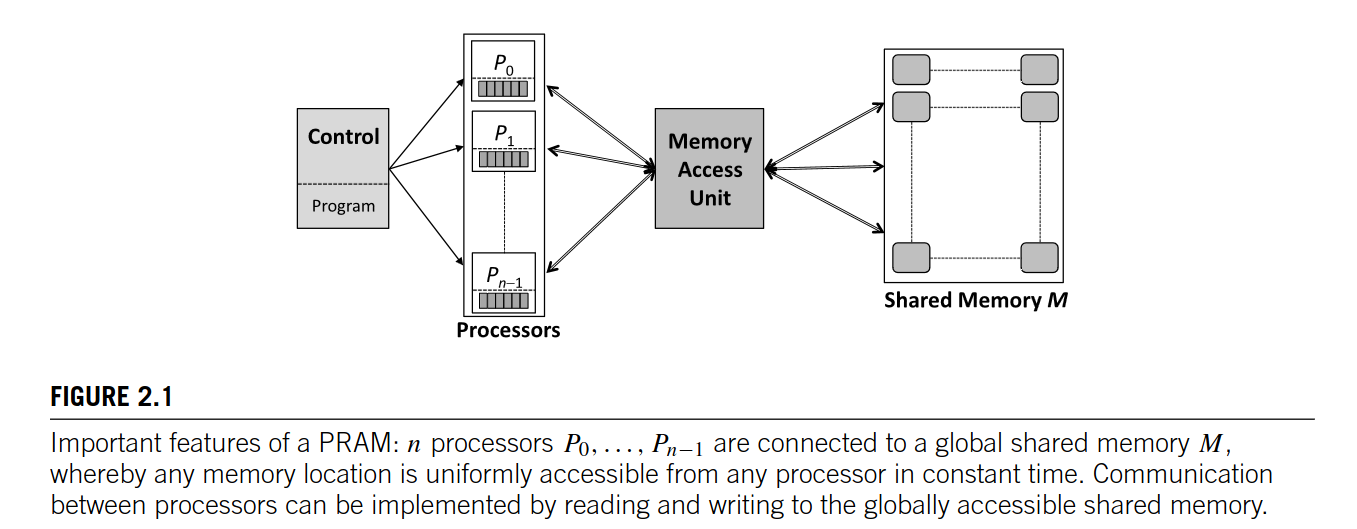
\includegraphics[width=0.9\textwidth]{Images/PRAM.png}
    \caption{PRAM Model}
\end{figure}

PRAM consists of $n$ identical processors $P_i$ for $0 \leq i \leq n-1$. In every step each processor executes an instruction cycle in three phases:
\begin{enumerate}
    \item \textbf{Read Phase:} Each processor can simultaneously read a single data item from a (distinct) shared memory cell and store it in a local register.
    \item \textbf{Compute Phase:} Each processor can perform a fundamental operation on its local data and subsequently stores the result in a register.
    \item \textbf{Write Phase:} Each processor can simultaneously write a data item to a shared memory cell,whereby the exclusive write PRAM variant allows writing only distinct cells while concurrent write PRAM variant also allows processors to write to the same location which can lead to race conditions.
\end{enumerate} 

Three phase PRAM instructions are executed synchronously. Communications between the processors in the PRAM needs to be implemented in terms of reading and writing to shared memory. This type of memory can be accessed in a uniform way; i.e., each processor has access to any memory location in unit (constant) time. This makes it more powerful than real shared memory machines in which accesses to (a large) shared memory is usually non-uniform and much slower compared to performing computation on registers. The PRAM can therefore be regarded as an idealized model of a shared memory machine; e.g. we cannot expect that a solution for a real parallel machine is more efficient
than an optimal PRAM algorithm.

\subsection*{PRAM Variants}
Several types of PRAM variants have been defined which differ in how data in shared memory can be read/written: only exclusively or concurrently. So we have 4 possible combinations
\textbf{ER} - Exclusive Read, \textbf{CR} - Concurrent Read, \textbf{EW} - Exclusive Write, \textbf{CW} - Concurrent Write. These are also shown in Figure 2.2.
We now describe three most popular variants the EREW, CREW, and CRCW PRAMs.

\begin{figure}[h]
    \centering
    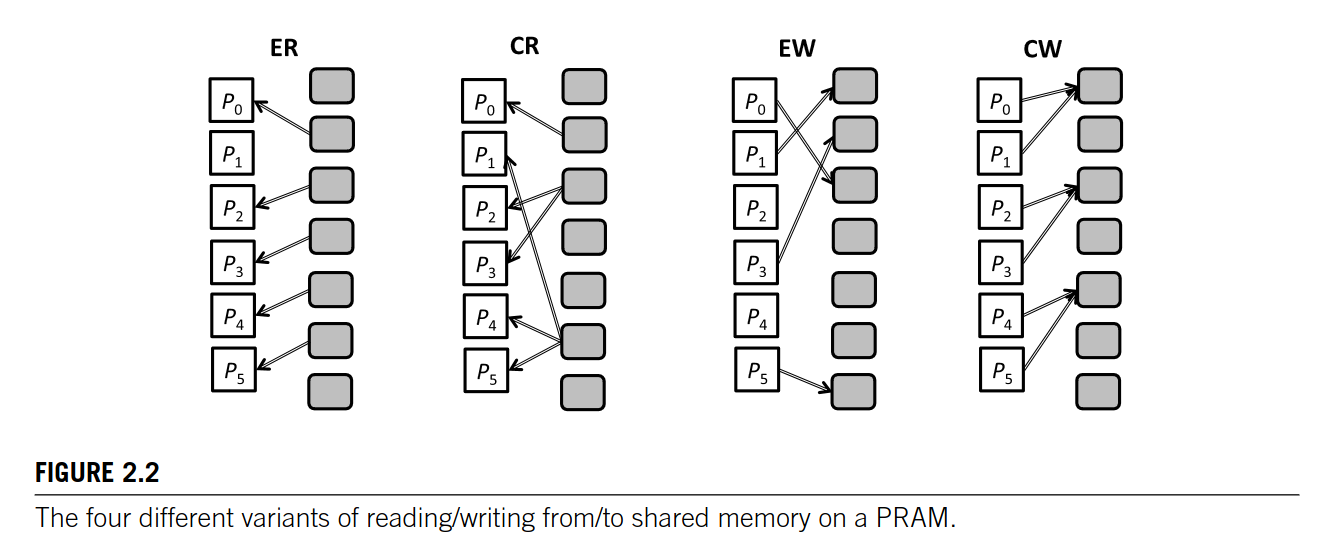
\includegraphics[width=0.9\textwidth]{Images/PRAM2.png}
    \caption{PRAM Variants}
\end{figure}

\subsection*{EREW PRAM}
EREW stands for Exclusive Read Exclusive Write. No two processors are allowed to read or write to the same memory location during same cycle.

\subsection*{CREW PRAM}
CREW stands for Concurrent Read Exclusive Write. Several processors may read data from the same shared memory cell simultaneously. Still, different processors are not allowed to write to the same shared memory cell.

\subsection*{CRCW PRAM}
CRCW stands for Concurrent Read Concurrent Write. Both simultaneous reads and writes to the same shared memory cell are allowed in this variant. In case of a simultaneous write (analogous to a race condition) we need to further specify which value will actually be stored. \\

There are 4 common approaches to deal with the situation where two or more processors attempt to write to same memory location during the same clock cycle are:
\begin{enumerate}
    \item Priority Concurrent Write (CW) - Processors have been assigned distinct priorities and the processor with the highest priority succeeds in writing its value to the shared memory.
    \item Arbitary Concurrent Write (CW) - A randomly choosen processor succeeds in writing its value to the shared memory.
    \item Common Concurrent Write (CW) - All processors writing to same global memory must write the same value.
    \item Combining Concurrent Write (CW) - All values to be written are combined into a single value by means of an associative binary operations such as sum, product, minimum, or logical AND.
\end{enumerate}

\subsection*{Parallel Prefix Sum Computation}
1. First method involves spawnning N threads and each thread computes one element of the prefix sum array. Here is simple CUDA kernel code for this one assuming that threads are distributed in such a way global thread ID $\leq N-1$.

\codebox{\textbf{Prefix Sum CUDA Kernel Implementation $\mathcal{O}(n^2)$}}

\begin{lstlisting}
__global__ void NaivePrefixSum(int* A, int* C) {
    int index = threadIdx.x;

    int sum = 0;
    for(int i = 0;i <= index; i++) {
        sum += A[i];
    }

    C[index] = sum;
}
\end{lstlisting}

\newpage

2. Second method is slightly better approach than first one and is easy to understand from followig figure

\begin{figure}[h]
    \centering
    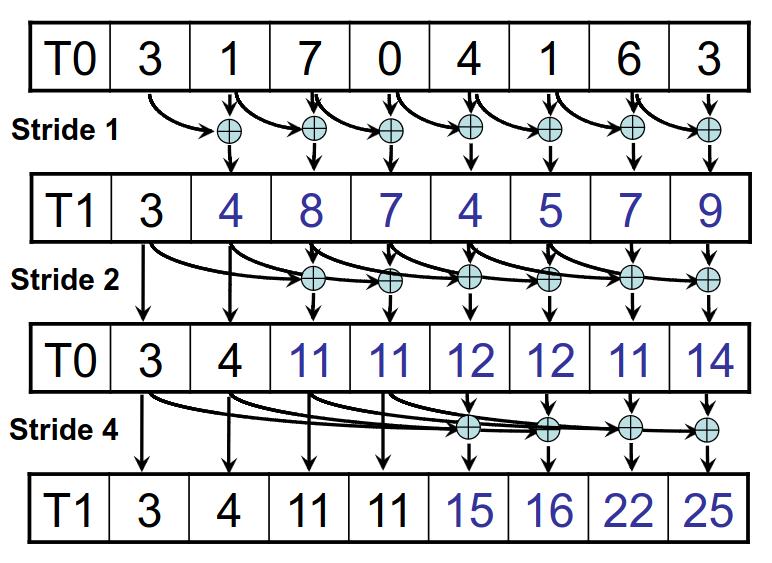
\includegraphics[width=0.6\textwidth]{Images/prefix2method.png}
    \caption{Prefix Sum Approach 2 $\mathcal{O}(nlogn)$}
\end{figure}

\codebox{\textbf{Prefix Sum Approach 2 $\mathcal{O}(nlogn)$}}

\begin{lstlisting}
__global__ void PrefixSum2(int* A, int* C, int N) {
    int index = threadIdx.x;
    for(int stride = 1; stride < N; stride *= 2) {

        if(index + stride < N) {
            C[index + stride] += C[index];
        }

    }
}
\end{lstlisting}

\subsection*{Parallel Merge of 2 Sorted Lists}
Normally merge of two sorted lists takes $\mathcal{O}(m+n)$ time and $\mathcal{O}(m+n)$ space. Where as if we have to do this in constant space then it will take $\mathcal{O}(mlogm + nlogn)$ time, Here in our parallel algorithm we will have $n$ processors for $n$ elements in first list and $m$ processors for $m$ elements in second list.

\begin{itemize}
    \item The processor knows index of element in own list.
    \item It then finds the index of element in other list using binary search.
    \item sum of these two indices gives the index of element in merged list.
    \item Write the element to this index in merged list.
\end{itemize}

Clearly we can see that the complexity is $\mathcal{O}(nlogm + mlogn)$. Here is the CUDA kernel code for this algorithm. This algorithm will only work if all elements in both lists are \textbf{distinct}.

\codebox{\textbf{Device Function for Binary Search}}

\begin{lstlisting}
__device__ int binarySearch(int* nums, int target, int N) {
    int lo = 0;
    int hi = N-1;
    int mid;
    while(lo <= hi) {
        mid = lo + (hi-lo)/2;
        if(nums[mid] == target) return mid;
        else if(nums[mid] < target) lo = mid+1;
        else hi = mid-1;

    }
    return lo;
}
\end{lstlisting}

\codebox{\textbf{Merge of 2 Sorted Lists CUDA Kernel}}

\begin{lstlisting}
__global__ void merge2SortedLists1(int* A, int* B, int* C, int N, int M) {
    int idx = blockDim.x * blockIdx.x + threadIdx.x;
    if(idx >= N+M) return;

    if(idx < N) {
        int otherIdx = binarySearch(B,A[idx],M);
        C[idx+otherIdx] = A[idx];
        printf("Idx = %d, otherIdx = %d for element %d \n", idx, otherIdx, A[idx]);
    }
    else {
        int otherIdx = binarySearch(A,B[idx-N],N);
        C[idx-N+otherIdx] = B[idx-N];
        printf("Idx = %d, otherIdx = %d for element %d \n", idx-N, otherIdx, B[idx-N]);
    }
}
\end{lstlisting}

\subsection*{Enumeration Sort}
This sorting algorithm takes $\mathcal{O}(n^2)$ comparisons, so we are going to spawn $n^2$ threads for each comparison and hence we can sort in $\mathcal{O}(1)$ time. Here is the algorithm for Enumeration Sort.

\begin{itemize}
    \item Each thread compares $a[i]$ and $a[j]$. If $a[i] > a[j]$ then $pos[i] = pos[i] + 1$.
    \item Threads will do concurrent write to $pos[i]$ and we used atomic add operations to put the sum of all increments in $pos[i]$.
    \item Finally we will have position of each element in sorted array.
\end{itemize}

\codebox{\textbf{CUDA Kernel Implementation for Enumeration Sort}}

\begin{lstlisting}
__global__ void EnumerationSort(int* A, int* POS) {
    int threadID = threadIdx.x;
    int blockID = blockIdx.x;

    if(A[threadID] > A[blockID]) {
        atomicAdd(&POS[threadID],1); // Ensures correct parallel addition
    }
}
\end{lstlisting}

\codebox{\textbf{Post Processing Step}}
This Post processing step is not needed if all the elements are distinct. If there are duplicates then we need to do this step.

\begin{lstlisting}
    // Initializing answer array to 0.
    int* answer = (int*)malloc(size);
    for(int i = 0;i < N; i++) answer[i] = 0;

    // Fill Elements at correct place
    for(int i = 0;i < N; i++) {
        int idx = pos[i];

        if(answer[idx] != 0) {  // This is case when duplicate elements are present
            int k = 1;
            bool flag = true;

            while(flag) {
                if(answer[idx+k] == 0) {
                    answer[idx+k] = answer[idx];
                    flag = false;
                }
                else k++;
            }
        }
        else answer[idx] = A[i];
    }
\end{lstlisting}
